\section{SEM - Scanning Electron Microscopy}
The electron microscopy is an instrument that allow us to create images/visualize organic and inorganic structures with impressive magnification.It is an invaluable instrument in the engineering and development of new materials where nano-meter sized imaging is very important. The SEM can also be used in chemical analysis and accessing the crystalline structures of materials. In comparison to light microscopy is the depth of field much larger in scanning electron microscopy thanks to the narrow electron beam. The resulting images get a 3D appearance due to this large field of depth that is very useful when examining the surface structures. 

\subsection{History}

\subsection{Operational steps}
The idea behind the technique is to generate a beam of energetic electrons with emission from an electron source. This is typically done by heating up a metal (Tungsten for example) in vacuum and accelerate the electrons with a electric field. The electrons are stopped from leaving the atoms of the metal be an energy barrier between the emission tip and the surrounding vacuum. By adding an electric field in the vacuum the energy barrier is reduced to a "slope", but the electrons still need to perform the "work" W to pass this barrier. Luckily there is an quantum effect called tunneling allowing electrons to tunnel through this barrier out into to vacuum.   

\textcolor{red}{Illustration of tunneling} 

There are several types of electron emitters (cathodes) with different properties being used in electron microscopy today. One of the older and cheaper options are the so called \textbf{W Hairpin} made of Tungsten. These are widely used in older SEM and TEM microscopes. Tungsten is used because of its high melting point and low vapor pressure. This makes it possible to electrically heat to make electron emission possible. Another option is \textbf{Lanthanum Hexaboride LaBa$_6$} which has a low work functions, meaning the energy to remove an electron from the metal to a point in the vacuum outside the metal is low. This type of cathode is about 10 times "brighter" then Tungsten cathodes \textcolor{red}{meaning?}. A third alternative is FEG \textbf{Field Emission gun} which can create a beam that is smaller in diameter and more coherent and up to three times greater magnitude of "brightness/current density" The FEG is sharply pointed with an emitter that is held at several kilovolts of negative potential energy compared to a nearby electrode. This makes the potential gradient sufficient to cause electron field emission.     



The energy of the electrons in this beam is measured in 1eV which is equivalent to what a electron in an electric field generated by 1 V would have. This energy is denoted $E_0$ and is often around 0.1 to 30keV. The electron beam is after acceleration modified/reshaped by lenses and apertures to reduce the diameter of the beam and to scan this beam into a raster of x-y coordinates which it sequentially is placed in. This coordinates are discrete but closely spaced. The lenses are no ordinary glass lenses since the electrons would pass through them or lose to much energy (wouldn't focus them either). Instead are they modified with electrostatic lenses and electromagnetic coils into desired shape and properties. 

When the primary electrons in the electron beam hit the specimen it interacts with it forming a interaction volume. The electron penetrate the specimen material and looses energy by random scattering and absorption this process with all electrons in the beam form a volume of interaction that is teardrop shaped. The interaction results in different types of electrons being emitted/scattered from the specimen. 

At each of the raster coordinates in the scan pattern are two types of outgoing electrons from the specimen created: \textbf{back-scattered electrons (BSE's)} and \textbf{secondary electrons (SE's)}. The BSE's are electrons that emerge from the specimen with a lot of the initial energy after interacting with the atoms electric fields of the atoms in the specimen, scattering and deflection. The SE's are electrons that emerge from the specimen surface after the electron beam have ejected them from the atoms in the sample. These electron escapes with very low energy compered to the typically high energy electron beam. They are in the range of 0-50eV with the majority below 5eV. 


The secondary electrons are often measured with a Everhart-Thornley detector that is sensitive for both SE's and BSE's while the BSE's are measured with a dedicated BSE detector that is not sensitive for the SE's. The signal for each of the detectors are measured at each of the coordinates in the x-y raster. The location and the intensity is recorded and correspond to a gray value in the x-y coordinates. Other sensors can also be used to capture for example X-ray signals that also can be emitted from the specimen due do the electron beam. 


\begin{figure}[ht!]
\centering
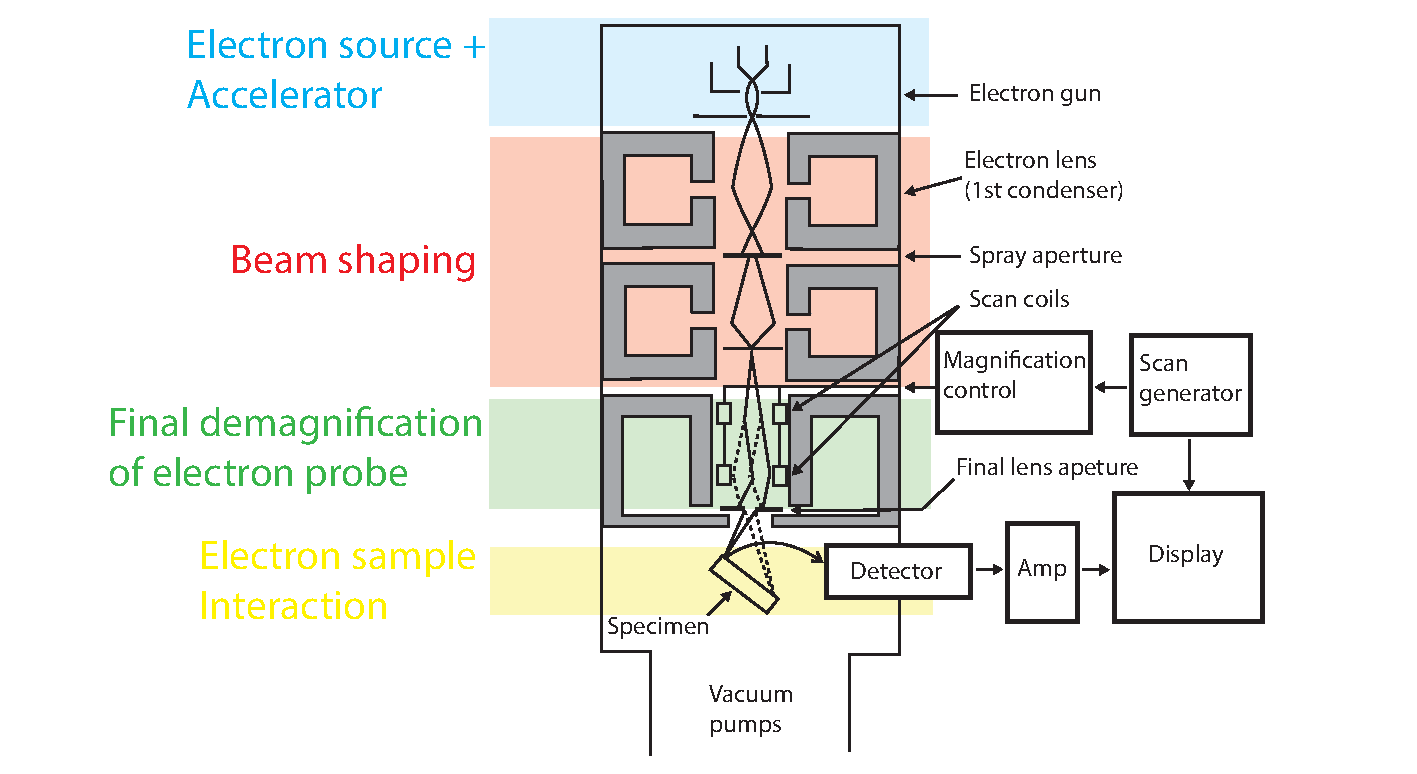
\includegraphics[width=120mm]{figures/Electron_microscopy.pdf}
\caption{Example of caption}
\label{fig:example}
\end{figure}


\subsection{Densitometric}
In order to create contrast between the different features of the sample there is need for a signal need to distinguish them. The BSE's and SE's give us different information about the specimen.

The physical property of being depicted in the imaging using BSE's are the mass of the atoms in the specimen/the chemical composition. Heavier atoms backscatter electron more strongly and they will therefore have more energy. Brighter spots on the image of BSE will therefore indicate areas with more heavier atoms. The contrast in the image is therefore used to identify areas with different chemical composition.

The secondary electron energy is linked to the incline of electron beam into the sample. If the beam enters the sample from an angle <90 degrees the interaction volume will be more exposed to the surface of the sample, making more SE's escape the specimen surface and being picked up by the detector. The SE's are counted and the increased number of them at inclines will give a brighter pixel in the digital image. 

Sample preparation is important for non-conductive samples since it is otherwise a risk that the electron beam will build up a charge on the surface of the sample. This charge will start to deflect the incoming electron beam making it impossible to scan the sample properly. By sputter a thin layer of conductive metal onto the specimen this can be avoided. Typically is gold, platinum and iridium. 

If an image is noisy or show low contrast then there have not been enough electron probe current to get a smooth noise-free image. 

calibration, scanning same "sensor" for all x,y coordinates of the sample, 

\subsection{Geometrical}
Scanning electron microscopy relates to the "real world" differently depending on if the information from BSE's or SE's are used. The energy of the BSE's are closely linked with the atomic number of the material the electron hits. The BSE's give an image of how the chemical composition is distributed over the specimen. Depending on the acceleration voltage used on the incoming primary electrons they penetrate differently deep before being backscattered. If the interest lies in the specimen surface it is important to use a acceleration voltage that make the primary electrons interact in the surface of the specimen. 

In the case of SE's are the energy of the electrons dependent on the inclination of the point in the sample/specimen were the electron beam is hitting. The different intensities of the SE's give topographic contrast imaging. This is caused by the interaction volume having more escaping electrons in the inclined case than the normal case.

The resolution or the smallest observable feature in a SEM image is typically around 0.5 - 1.5 nanometers. This resolution depends on several things, including electron beam size and the interaction volume with the specimen. The beam size can be controlled with an aperture or with the condenser lenses but this has an negative effect on the beam current resulting in long exposure times. The resolution can be increased by reducing the wavelength by increasing the acceleration voltage. When increasing the acceleration voltage one must keep in mind that the electrons will penetrate deeper into the specimen before reflecting back as BSE's generating more SE's on the way. This will make it impossible to get a detailed image of the surface of the specimen. It is also an increased risk of surface charging if the specimen is not conducting. Building up charge on the surface will deflect the electron beam making it hard to get a clear image. Pre-treatment can be used to avoid this phenomenon. An image with BSE's has lower resolution since they originate from deeper within the sample. 

The focus of a scanning electron microscope is intended to where the electron beam has the smallest diameter as it improves the resolution. When making the beam narrower it increases the angle of the cone of where the focal plane is. The increase in this angle makes the depth of field shorter. In SEM imaging the depth of field can be increased from a few microns to several millimeters. 


Distortions such as astigmatism in the resulting image is the result of imperfections in the lens system. When increasing the magnification the effect get more apparent. The resulting image distorts round shapes so that they appear elliptical. This can be corrected for by manually (or use the automated correction) adjusting the stigmator control in order to get better results. 

\subsection{Spectral}

SE's BSE's X-ray

\subsection{Temporal}
Exposure time, sample size, electron beam diameter, 






